% !TeX spellcheck = en_GB
\documentclass{article}
\usepackage{hyperref}
\usepackage{amsmath}
\usepackage{amssymb}
\usepackage{pgfplots}
\usepackage{float}
\usepackage{todonotes}
\usepackage{tikz}
\usepackage[shortlabels]{enumitem}

\renewcommand{\Re}{\mathbb{R}}
\newcommand{\Li}{\mathcal{L}}
\newcommand{\Ex}{\mathbb{E}}
\renewcommand{\Pr}{\mathbb{P}}
\newcommand{\Hy}{\mathcal{H}}
\newcommand{\sign}{\text{sign}}
\newcommand{\error}{\text{error}}

\newcommand\bigO[1]{
    \ensuremath{\mathcal{O}\left(#1\right)}
    }

\newcommand{\sigmoidPlot}{
    
    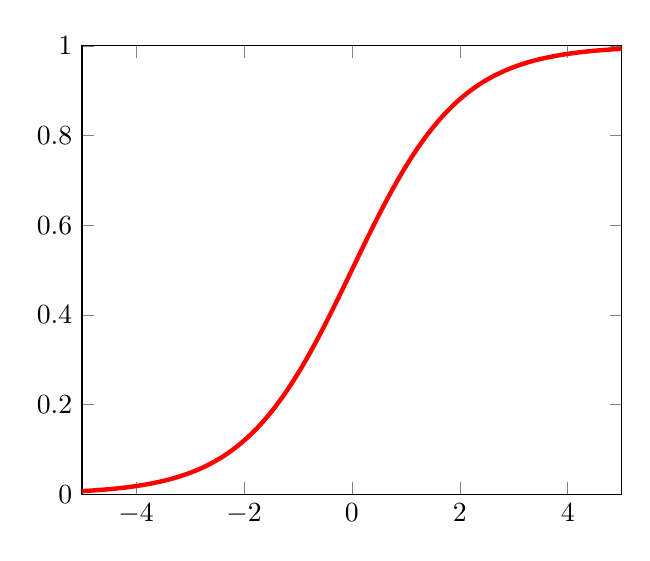
\begin{tikzpicture}
        \begin{axis}[xmin=-5, xmax=5, ymin=0, ymax=1, samples=150]
        \addplot[red, ultra thick] {1/(1+exp(-x))};
        \end{axis}
    \end{tikzpicture}
    
    }

\usetikzlibrary{positioning, calc}
\usetikzlibrary{arrows.meta}

\tikzstyle{circlebox}=[circle,thick,draw=black!75,minimum size=8mm]
\tikzstyle{inputnode}=[circlebox, draw=blue!75]
\tikzstyle{hiddennode}=[circlebox, draw=orange!75]
\tikzstyle{outputnode}=[circlebox, draw=orange!75]
\tikzstyle{simplebox}=[rectangle,thick,draw=black!75,
fill=black!20,minimum size=4mm]
\tikzstyle{textbox}=[rectangle,thick,minimum size=4mm,draw=black!0,
fill=black!0]
\tikzstyle{halfvdistance}=[yshift=-0.7cm]
\tikzstyle{abovebetween}=[xshift=-2.7mm]
\tikzstyle{edgepath} = [-Latex,->,shorten >=1pt,-stealth,semithick, rounded 
corners=5pt]

\def \nodedv {0.735cm}
\def \nodedh {0.65cm}

\tikzset{
    between/.style args={#1 and #2}{
        at = ($(#1)!0.5!(#2)$)
    }
}
\begin{document}
	\frontmatter
	\maketitle
	
	\tableofcontents*
	
	\mainmatter
	
	\chapter{General}
	
	\section{Degrees of P2P Structure}
	\begin{itemize}
		\item Unstructured networks
		\item Semi-structured networks
		\item Structured networks	
	\end{itemize}
	
	\todo{Compare types of network}
	
	\section{P2P Characteristics}
	\begin{itemize}
		\item Scalability
		\item Performance
		\item Availability
		\item Fairness
		\item Integrity and authenticity
		\item Security
		\item Anonymity, deniability and censorship resistance
	\end{itemize}
	
	\chapter{Unstructured P2P networks}
	
	\section{Napster}
	Single point of failure in its lookup- / index-server.
	
	\section{Gnutella}
	\begin{itemize}
		\item The first major truly distributed P2P network.
		\item Quite primitive, yet hugely successful
	\end{itemize}
	
	\subsection{Commands}
	\begin{itemize}
		\item[Ping] Ask for information about a peer.
		\item[Pong] The response to a Ping.
		\item[Query] Ask for the address for some information.
		\item[QueryHit] The response to a query.
	\end{itemize}
	
	\texttt{QueryHits} follow the query-route back to its originator.
	
	Queries have a \gls{UID}, and a \gls{TTL} to make sure that the same query is not re-transmitted and that queries die out.
	
	\subsection{Drawbacks}
	Peers report:
	\begin{itemize}
		\item Amount of shared data.
		\item Available bandwidth.
	\end{itemize}
	Self reporting lead to free-loaders.
	
	Flooding generates a lot of duplicate network traffic, Gnutella can swamp the network, even without any data-traffic. You could use Ring instead, but it has a worse worst-case.
	
	Downloads the whole file from a single peer, so if that peer dies, so does your file-transfer.
	
	\section{k-Walkers}
	A walker: A query traverses the network randomly, until a match is found. $k$-Walkers is simply having $k$ queries traversing.
	
	Much more efficient in terms of traffic, user-perceived delay is longer.
	
	Variations: $Maintain state$, and do not forward the same query to the same neighbour twice. $Check$ source for sufficient success. $Check$ visits fewer nodes than the other variation.
	
	\subsection{Results}
	Scales much better than flooding. Increased user-perceived delays. Blindly using \gls{TTL} is inefficient. Queries should check back.
	
	\textbf{However} simulation assumes a stable network, and it may not be distributed in a nice way.
	
	\section{Gia}
	A system combining:
	\begin{itemize}
		\item \textbf{Topology adaptation} - peers should connect to strong and well-connected peers able to handle the traffic.
		\item \textbf{Active flow control} - if a peer is overloaded it should not be bothered until it is ready again.
		\item \textbf{One-hop replication} of indices - every peer knows what its neighbours store.
		\item \textbf{Biased random walking} - queries seek towards high capacity peers.
	\end{itemize}
	
	\subsection{Terms}
	\begin{itemize}
		\item[Capacity] ability to handle messages/time - i.e. bandwidth, CPU power etc.
		\item[Satisfaction] $0\dots1$: degree to which a peer's own capacity is matched by the sum of its neighbours' capacities/degree.
	\end{itemize}
	
	
	\subsection{Adaptive flow control}
	Peers sends tokens to its neighbours according to its (and their) capacity. Peers only sends queries to other peers if they have a token from that peer. So if they claim to have a low capacity, the other peers will send it fewer tokens, which they need in order to get work done.
	To reduce overload, publish fewer tokens and queue queries.
	
	\subsection{One-hop replication}
	Peers maintain indices over their neighbours' resources. Query results will contain a pointer to the resource, not the index. This evens the load for peers with many resources. 
	
	\subsection{Biased random walking}
	Walkers will walk towards the strongest peers in the hub. I.e. peers will direct it to the node with the highest capacity tokens.
	
	\chapter{Structured P2P networks}
	
	\section{Distributed hash tables}
	Assign peers evenly across an ID-space.
	
	Assign resource IDs in the same ID-space. Resources are associated with the following (in ID-space) peer.
	
	Searching for a resource and for a peer becomes the same thing.
	
	\section{Chord}
	One operation: \texttt{address = lookup(key);} Given a key, find a node responsible for that key.
	
	\subsection{Goals}
	\begin{itemize}
		\item Load balancing
		\item Decentralization
		\item Scalability
		\item Availability
		\item Flexible naming
		\item Lookup in \bigO{\log(n)}
		\item Each node needs information about \bigO{\log(n)} peers
	\end{itemize}
	
	\subsection{Hashing in Chord}
	A good hash function balances load (uniformly distributes them). Even small changes, results in big differences in hashes. Cryptographic hashes, such as SHA-256, is very hard to get the key from the hash. 
	
	Big enough space to make collisions improbable.
	
	\subsection{Node leaving}
	All of node $n$'s keys are assigned to \texttt{successor(n)}.
	
	\subsection{Node joining}
	Keys $k \leq n$ assigned to \texttt{successor(n)]} are assigned to $n$. A physical node may run any number of peers on different ports.
	
	\subsection{Key location}
	\textbf{Linear:} takes \bigO{n} time, and \bigO{1} space.
	\\
	\textbf{Scalable:} use fingertables, point to the $2^{i-1}$ next node. $\text{n.finger}[i] = \text{find\_successor}(n+2^{i-1}), 1 \leq i \leq m$.
	
	Simply find the node $n'$ in the fingertable, which is closest to the key. This node will be the one in the fingertable, that will know most about $n'$.
	
	\subsection{Successor lists}
	If a node fails, use successor list of size $s$ to re-establish the network.
	
	\subsection{Conclusion}
	\begin{itemize}
		\item Based on distributed, consistent hashing.
		\item Performance and space is \bigO{\log(n)} for stable networks.
		\item Simple, provable performance and correctness.
		\item Too simple, does not consider locality or strength.
	\end{itemize}
	
	\section{Pastry}
	\begin{itemize}
		\item Effective: \bigO{\log(n)} routing hops.
		\item Distributed: no servers, and limited knowledge at nodes (\bigO{\log(n)} routing table sizes).
		\item Substrate: Not an application, rather an \gls{API} to be used by applications.
		\item NodeId: similar to Chord.
	\end{itemize}
	
	\subsection{API}
	\begin{itemize}
		\item \texttt{nodeID = pastryInit(Credentials, Application);}
		\item \texttt{route(msg, key);} routes a message to the live node, with its ID numerically closest to the key.
		\item (Callback, application implements) \texttt{deliver(msg, key);} called on the application at the destination node for the given id.
		\item (Callback, application implements) \texttt{forward(msg, key, nextId);} called on the application, when the node is about to forward the given message to the node with $nextId$ as id.
	\end{itemize}
	
	\subsection{Assumptions and guarantees}
	Routes messages in $\log_{2^b}(n)$ steps. Where $b$ is the base the id's are in.

	Unless $\lvert L \rvert / 2$ adjacent nodes fail concurrently, eventual delivery is guaranteed. ($\lvert L \rvert$ being a configuration parameter).
	
	Join and leave in \bigO{\log(n)}.
	
	Maintains locality, based on application-defined scalar proximity metric.
	
	\subsection{Routing table}
	3 parts, \texttt{Leaf Set}, \texttt{Routing Table} and \texttt{Neighbourhood Set}.
	
	\subsubsection{Leaf Set}
	Contains the $\lvert L \rvert$ numerically closest smaller nodeIds, as well as the $\lvert L \rvert$ numerically closest larger nodeIds.
	
	\subsubsection{Routing Table}
	Has \texttt{ceiling}$(\log_{2^b}(N))$ rows with $2^b-1$ entries. 
	
	Each entry in row $n$ shares a prefix of length $n$ with the current node.
	
	\subsubsection{Neighbourhood Set}
	$\lvert M \rvert$ closest nodes according to proximity metric. ($M$ begin a configuration parameter).
	
	\subsection{Routing in Pastry}
	The node first checks if the key is within the range of the \texttt{Leaf Set}. If not, it uses the routing table to forward the message to a node that shares a common prefix with the key by at least one digit.
	
	In the rare case that the appropriate entry is empty or unreachable, then the message will be forwarded to some known node, with a prefix at least as good as the current node, and is numerically closer.
	
	\subsection{Node joining}
	A new node, $n$ has to know about some nearby node $m$. $n$ asks $m$ to route a "join" message with key equal to $n$. \texttt{Pastry} then routes this message to node $p$ with the nodeId numerically closest to $n$. All nodes on the route to $p$ returns their state to $n$.
	
	$n$ updates its state, based on returned state:
	\begin{itemize}
		\item \texttt{Neighbourhood Set} = \texttt{Neighbourhood Set} of $m$.
		\item \texttt{Leaf Set} is based on \texttt{Leaf Set} of $p$, since $p$ is numerically closest to $n$.
		\item Rows of the \texttt{Routing Table} are initialised based on the nodes visited on the route to $p$, since they share increasing common prefixes with $n$.
	\end{itemize}
	
	$n$ then calibrates its \texttt{Routing Table} and \texttt{Neighbourhood Set} based on data from the nodes referenced therein. 
	
	$n$ sends its state to all the nodes mentioned in its overall routing table. In total, \bigO{\log_{2^b}(n)} messages exchanged. (Since that's amount of nodes visited in the join message).
	
	\subsection{Locality}
	Applications are responsible for providing proximity metrics. Pastry assumes the triangle inequality holds.
	
	\subsection{Node failure}
	\subsubsection{Leaf Set}
	\begin{itemize}
		\item Contact the live node with the largest index on the side of the failed node, and get leaf set from that node.
		\item Returned leaf set will contain an appropriate node to insert.
		\item This works, unless $\lvert L \rvert$ adjacent nodes have failed.
	\end{itemize}
	
	\subsubsection{Routing Table}
	\begin{itemize}
		\item Contact other node on the same row, to check if this node has a replacement node (the contacted node may have a replacement node on the same row of its routing table).
		\item If not, contact node on next row of routing table.
	\end{itemize}
	
	\subsubsection{Neighbourhood Set}
	\begin{itemize}
		\item Neighbourhood set is normally not used in routing, therefore contact periodically to check liveness.
		\item If a neighbour is not responding, check with live neighbours for other close nodes.
	\end{itemize}
	
	\section{Kademlia}
	Routing done by halving the ID-space distance in each routing step. Similar to the \texttt{Routing Table} in Pastry's routing table.
	
	Routing done in \bigO{\log(n)}, space used is \bigO{\log(n)}.
	
	\subsection{Critique of other systems}
	\begin{tabular}{p{0.5\textwidth} | p{0.5\textwidth}}
		\textbf{Chord}:
		\begin{itemize}
			\item Fingertables only forward looking
			\item Messages arriving at peer tells it nothing useful, knowledge must be gained explicitly
			\item Seperate track of control message exchanges
			\item Rigid routing structure
			\item Locality difficult to establish
		\end{itemize}
		&
		\textbf{Pastry}:
		\begin{itemize}
			\item Complex routing algorithm
			\item First routing table, then leaf set
			\item Maintains three different tables: leaf, routing and neighbour
		\end{itemize}
	\end{tabular}
	
	\subsection{IDs}
	All IDs are 160 bits long, found using a uniform distribution function, such as SHA-256. Kademlia uses xor to navigate this ID space. $d(X, Y) = X \text{ XOR } Y \implies d(X, Y) = d(Y, X)$
	
	Intuition: The more significant the different bits are, the longer distance there are between them.
	
	\subsection{Routing table}
	A Kademlia routing table, stores 160 k-buckets. The $i^{th}$ k-bucket, contains nodes within a \texttt{XOR} distance of $2^i$ to $2^{i+1}$ from itself (so the $i^{th}$ bit is significant).
	
	There can be up to $k$ nodes in each bucket, ordered by liveness (most recently seen are positioned at tail). So they have finest grained knowledge about the closest peers, and coarser knowledge about the rest of the world.
	
	\subsection{Commands}
	\begin{itemize}
		\item[Ping] check if a peer is still alive.
		\item[Store] store some key-value pair at the peer.
		\item[Find\_Node] Returns the $k$ closest nodes to an ID, that the peer knows.
		\item[Find\_Value] Similar to \texttt{Find\_Node} but if the node knows the value, it returns the value instead. If one of the $k$ closest nodes does not have the value, the requester will store it there.
	\end{itemize}
	
	\subsection{Maintenance of routing tables}
	Maintenance is ongoing, when communication with another node happens:
	\begin{itemize}
		\item Check the appropriate $k$-bucket.
		\begin{itemize}
			\item If already there, move to tail.
			\item If there is room, insert at tail.
			\item If unknown, and least recently seen node is unresponsive (at the head), replace with new node (and move to tail).
			\item Otherwise, do nothing.
		\end{itemize}
	\end{itemize}
	Over time, this means that old peers will stay in the buckets, as long as they are alive. This indirectly favors old peers that have stayed in the buckets for a long time (e.g. $k$ old peers in one bucket, will never be replaced by a new peer if they stay alive). The longer a peer stays online, the higher the probability is that it will remain online.
	
	Protects from flooding with bogus peers.
	
	\subsection{Parallelism}
	In Kademlia, we can send queries to multiple nodes, and just use the response from the quickest node. This prevents one peer from slowing bottle-necking the network.
	
	\subsection{Redundancy}
	Data expires after 24 hours, so original publisher has to republish every 24 hours to maintain information. Each (key,value) pair is stored at $k$ locations close to the key.
	
	Whenever a peer $A$ observes a new peer $B$ with ID closer to some of $A$'s keys, $A$ will replicate these keys to $B$.
	
	\subsection{Joining the network}
	\begin{itemize}
		\item Compute an ID
		\item Somehow locate a peer in the network
		\item Add the peer to the k-bucket
		\item Find neighbours with \texttt{Find\_Node} on own ID
		\item Populate the other k-buckets by performing \texttt{Find\_Node}
		\item Since we issue queries on other nodes, those nodes will implicitly be added to the appropriate $k$-buckets for these nodes.
	\end{itemize}
	
	\subsection{Failure}
	Unlikely, as routing tables are maintained by ordinary traffic. If there is no traffic, a peer will regularly refresh oldest k-bucket to keep updated.
	
	Parallelism in queries will ensure that a failing peer is both detected and bypassed.
	
	
	\chapter{The Internet of Things}
	
	\section{What is the IoT}
	The \gls{IOT} is 3 main parts:
	
	\begin{itemize}
		\item Identity - RFID, QR, MAC-address
		\item Connectivity - How can we address the object? Bluetooth, WiFi, IR etc.
		\item Capacity
		\begin{itemize}
			\item Simple: Identification
			\item Intermediate: Sensing
			\item Advanced: Reacting
		\end{itemize}
	\end{itemize}
	
	\section{What can we use it for}
	Logistics, intruders, smart homes etc.
	
	\section{Challenges}
	\begin{itemize}
		\item Energy usage
		\item Lack of IP Addresses. 32 bit not enough anymore, IPv6 = 128 bit
		\item Lack of standards, how are devices found, named, how are their abilites discovered etc.
		\item All major players are running with their own solution, no one is big enough to be the standard.
	\end{itemize}
	
	\subsection{Data silos}
	\begin{itemize}
		\item Pre-Web internet: Data flowed evenly between hosts.
		\item Present internet: Data flows from content-providers to end-users; data about habits collected.
		\item Future IoT internet: Countless sensors and devices, streaming data to central repositories (clouds).
	\end{itemize}
	Being the owner of the standard cloud service for \gls{IOT} is a major opportunity for a lot of big players, as they get access to all that data.
	
	\subsection{Security}
	A "smart" home, is a hackable home.
	
	\section{The Web of Things}
	A proposal for a solution, use the already existing platform, the \gls{WWW}, and use the existing protocols.
	
	\begin{itemize}
		\item GET
		\item PUT
		\item POST
		\item DELETE
	\end{itemize}
	
	\section{Disadvantages}
	\begin{itemize}
		\item HTTP is heavy.
		\item HTTP was not designed for streams.
		\item Security and discovery are both issues we can handle, but has to be handled explicitly.
	\end{itemize}
	
	\chapter{Security and privacy in P2P and the Internet of Things}
	
	\section{Dangers of distributed systems}
	\begin{itemize}
		\item Trust - Who can you trust?
		\item Identity theft - Pretending to be you or someone you trust
		\item Privacy - Preventing others from listening in on the conversation
		\item Censorship and attacks - Denying you the right to know
	\end{itemize}
	
	Data travels through numerous computers before it gets to the destination. This means data can always be intercepted, so we need make sure the interceptor cannot read it, as it will be useless to him.
	
	\section{Attacks agains distributed systems}
	
	\subsection{DDoS}
	Simply overload the system, often with a botnet.
	
	As \gls{DDOS} attacks usually focus on overloading one peer, and not all the peers at once. We should focus on how to protect single peers, and protect the network from losing a single peer.
	
	\textbf{Defences:}
	\begin{itemize}
		\item Minimize cost of losing \textit{any} peers.
		\item Make it difficult to identify the most important peers, so the attackers will have a hard time targetting them.
		\item Optimise traffic so it only affects a minimal part of the network.
		\item Prevent bogus data from overwriting good data.
	\end{itemize}
	
	\subsection{Malicious peers}
	Peers that reroutes data in the wrong way, poisons routing data for other peers, corrupts data etc.
	
	\textbf{Defences:}
	\begin{itemize}
		\item Do not rely on just one query route.
		\item Continuously very peers and data.
		\item Favour long living peers.
	\end{itemize}
	
	\subsection{Sybil attack}
	Creating \textbf{a lot} of fake peers and making them join the network, easy to do if one machine can masquerade as many.
	
	Allows surveillance or manipulation of traffic.
	
	\textbf{Defences:}
	\begin{itemize}
		\item Make joining expensive, so it is harder to do from a single machine.
		\item Make sure that paths on the overlay network involve multiple subnets, as sybil attacks are likely to originate from the same subnet, so involving multiple subnets can mask who the sender and receiver is.
	\end{itemize}
	
	\subsection{Eclipse attacks}
	Good peers are eclipsed by evil peers, that insert themselves between good peers and the network, cutting the good peers off from the network.
	
	\textbf{Defences:}
	\begin{itemize}
		\item Prevent peers from choosing their position in the network.
		\item Don't rely on a single path through the network.
	\end{itemize}
	
	\section{Techniques for anonymity and censorship resistance}
	
	\subsection{Crowds}
	This aims to defeat network tracking.\\
	Redirect requests through a number of random peers, before doing the request.
	
	Obscure who sent the request.
	
	\subsection{Mix networks}
	This aims to defeat traffic analysis.\\
	Send messages through a number of mixers $m_1 \dots m_n$, and encrypt the message with $m_n$'s \gls{PK}, then $m_{n-1}$ \gls{PK} down to $m_1$.
	Only $m_1$ knows the sender, and only $m_n$ knows the receiver and neither knows the route of the message nor their position on the path.
	
	\textbf{Issues:}
	\begin{itemize}
		\item Easy to block established mixers.
		\item Malicious mixers can recognize sender and recipient at that point.
		\item Doesn't protect the edges of the cloud (entering and leaving the mix network).
		\item It becomes feasible, but expensive to do edge traffic analysis.
	\end{itemize}
	
	\subsubsection{Tarzan}
	An attempt to fix the issues with existing mix networks.
	
	\begin{itemize}
		\item It's P2P - everyone can be a mixer, therefore hard to block all the mixers.
		\item Fake "cover" traffic, makes it hard to distinguish real traffic from the idle chattering.
		\item Cover traffic is sent at a uniform rate, and lowered when real traffic comes, so there wont be an increase in traffic.
		\item Peers must be validated, and you cannot fake your IP return address.
		\item Tarzan spreads traffic across the internet, so malicious peers can't make a lot of virtual peers.
	\end{itemize}
	
	\subsection{Freenet}
	A distributed filesystem, peers contribute diskspace and only a file-owner can alter a file.
	
	There is end-to-end encryption, and only the originator of a query knows it is the originator. Query results (files) are returned along the same route, during which peers might cache the file and claim that they are the data-holders. Thus hiding the actual data-holder from attacks. Peers might also alter the \gls{TTL}, to avoid \gls{TTL} analysis.
	
	Popular resources  are then replicated over the network, making \gls{DDOS} attacks self-defeating as the more you attack a resource, the more that resource is spread across the network.
	
	\subsubsection{Joining}
	Create a \gls{GUID} by hashing the resource, and send it out on the network with a \gls{TTL}. Unpopular files might be reclaimed by the system, to make room for popular files.
	
	\section{Securing DHT's}
	
	\textbf{Vulnerabilities}
	\begin{itemize}
		\item Deterministic routing
		\item Routing information kept at peers
		\item ID determines position
		\item Values kept at peer with closest key
	\end{itemize}
	
	\subsection{Kademlia}
	\textbf{Weaknesses}
	\begin{itemize}
		\item Deterministic routing along converging path
		\item Sybils can saturate the network with malicious peers
		\item Eclipse peers can work together to create poor routing
	\end{itemize}
	
	\textbf{Strengths}
	\begin{itemize}
		\item Prefers long living peers, so churn attacks will be inefficient
		\item Routing information is continually refreshed, there is no specific operation that can be targeted
	\end{itemize}
	
	
	\subsection{Securing Kademlia}
	Everybody has public/secret keys
	
	Securing Kademlia through:
	\begin{itemize}
		\item Expensive nodeId generation
		\item Sibling broadcast
		\item Ensuring that when we search for ID's we search across disjunct paths
		\item Verifiable messages
	\end{itemize}
	
	\subsubsection{Secure Node Identifiers}
	Sybils rely on cheap, home-made, unverifiable nodeId generation.
	\begin{itemize}
		\item ID's created as public-key hashes
		\item Weak signatures on just (IP,port,timestamp) for \texttt{PING, FIND\_NODE} commands.
		The timestamp will avoid replay attacks.
		
		\item Strong signatures on the whole message to avoid man-in-the-middle attacks, also include a nonce to avoid replays.
	\end{itemize}
	
	\textbf{Generating ID's}: If we have a central authority, it can control the ID-generation and limit the growth of Sybil's. But having a \gls{SPOF} is a bad idea, as it is contrary to the whole point of our \gls{P2P} network.
	
	\textit{Alternative:} Security by difficulty, use crypto-puzzles to make it computationally hard to create a nodeId. 
	
	This could be that for the generated $key$: $c_1 \text{ first bits of } H(H(key)) = 0$ which means we have to generate a lot of keys before we get our public key. Then it becomes computationally infeasible to generate a nodeId with a hash that gets placed between two specific nodes.
	
	To make it even harder, we add a $c_2$ and demand that the peer creates a $X$ such that  $c_2 \text{ first bits of } H(key \oplus X) = 0$, then we can increase $c_2$ over time to keep nodeId generation expensive.
	
	Verification is \bigO{1} while creation is \bigO{2^{c_1} + 2^{c_2}}.

	Ordinary peers just have to solve the puzzle once, but in Sybil attacks, you have to solve it thousands of times which is very expensive.
	
	\subsubsection{Sibling broadcast}
	Standard Kademlia has $k$ buckets and $k$ replicas of key/values \textit{(siblings)}. This marries network connectivity to redundancy.

	In the secure Kademlia, we instead have $s$ replicas of key/values.
	\todo{Unclear}
	
	\subsubsection{Populating the k-buckets}
	If you are able to provide a signed response, and if there is room in $k$-bucket, you can be added.
	
	Only adds valid (signed) nodeIds if the prefix is sufficiently different.
	\todo{Unclear}
	
	\subsubsection{Querying in S/Kademlia}
	Instead of just using the peer that answered quickest, it divides the $k$-peers into $d$-groups. Each of these groups, searches for the query as usual, with the exception that, if a group has visited a peer, the other groups will not visit this peer. This means their paths are disjoint. 
	
	This will reduce the likelihood that the whole query gets poisoned. It's important to note that it is not impossible for the whole query to get poisoned, but it is just a lot more expensive than ordinary Kademlia.
	
	\subsubsection{Conclusion}
	Making attacks harder by:
	\begin{itemize}
		\item Making nodeId generation harder with Crypto-puzzles.
		\item Accepting only signed nodeId's into $k$-buckets.
		\item Distributing queries across a wider set of the network.
	\end{itemize}
	At the cost of having good peers solve crypto-puzzles. (Joining takes longer).
	
	\section{Securing the Internet of Things}
	A lot of devices, involving a lot of different systems, architectures solutions and actors. What could possibly go wrong?
	
	What if someone hacks our water-supply, or the lock to my door?
	
	\subsection{Types of attacks}
	\begin{itemize}
		\item \gls{DDOS} - annoying if I can't use my toaster, catastrophic if the power-grid goes down.
		\item Surveillance - by companies, criminals or even the state.
		\item Intrusion - if one device gets hacked, it could potentially compromise all devices within the network. E.g. circumventing a firewall
	\end{itemize}
	
	\subsubsection{Network level security}
	\textbf{Different types of devices}:
	\begin{itemize}
		\item Strong cryptography simple to implement on ordinary computers, what about smaller simpler devices?
		\item Public key infrastructure may be difficult to handle in a larg \gls{IOT} setting.
		\item Gateways is a possible solution, the gateways handle the security and the things can keep doing what they do.
	\end{itemize}
	A centralistic solution is simple, but that is a \gls{SPOF} and if that is hacked then it will grant access to all the devices.
	\todo{Unclear}
	
	\subsubsection{Privacy}
	\begin{itemize}
		\item Unless we can ensure that the users data belongs to the user, then \gls{IOT} could become the perfect surveillance infrastructure.
		\item Gathering the users data at one point on the internet (centralistic) makes it easier to exploit.
		\item Distributed solutions keeps data closer to the user, so all the data isn't gathered in one place, and forces attacks to be targeted personally at a user.
	\end{itemize}
	
	\subsubsection{Identity}
	\begin{itemize}
		\item \gls{IOT} objects must have identities that can be found and authenticated by other services.
		\item Easy to implement in a centralised system, but in a distributed system, having a coherent namespace is challenging, as devices join and leave.
	\end{itemize}
	
	\subsubsection{Trust}
	\begin{itemize}
		\item Between the user and the system
		\item Also between devices, how does devices know that they can trust each other?
	\end{itemize}
	
	\subsubsection{Fault tolerance}
	\begin{itemize}
		\item Systems must cope with failures, things will go wrong with high amount of devices.
		\item Identify errors and failing sensors. Automatically choose alternate sensors or services.
		\item Identify compromised systems, and route around them if they are under attack.
	\end{itemize}
	
	\section{Conclusion}
	With the \gls{IOT} we get all the security and legal issues possible. Both technical issues, protection from hacking and attacks as well as the question of who owns the data? The provider of the service, the provider of the device etc..
	\todo{Could add more here, about security benefits between IOT and central}
	
	\chapter{Mobile ad hoc networks}
	Ad-hoc networks are small local networks for devices to communicate with eachother, as opposed to connecting to the "standard" network, such as the internet.
	
	Useful if, for some reason, one doesn't want to use the standard network. It might be expensive, slow or not available (or for any other reason).
	
	\section{Radios}
	Radios is by far the most common wireless communication technique. It has some issues:
	\begin{itemize}
		\item Signal strength diminishes with distance, and may vary a lot and seemingly unpredictably.
		\item Can be unidirectional
		\item Signals can be blocked by environmental factors, like walls, mountains or even rain.
		\item Signals are always broadcast, can be security problem but can also be an optimization.
	\end{itemize}
	
	\section{Routing}
	The issue with finding the "cheapest" path between devices. There might be a delay or cost for sending a packet from A to B, that is smaller if we send it from A to C to B. This could be because of environmental factors. 
	
	\subsection{Wired networks}
	Implementation through actual wires.
	\begin{itemize}
		\item Nearly static configuration.
		\begin{itemize}
			\item Nodes stay in the same place for a long time.
			\item Interconnecting links exist for an extended period of time.
		\end{itemize}
		\item Small fluctuations in link quality - usually only fluctuates when very high traffic rates are experienced.
		\item High traffic rates - there's usually a lot more communication going on in these types of systems.
	\end{itemize}
	
	\subsection{Classical routing approaches}
	\begin{itemize}
		\item Link State protocols
		\item Distance Vector protocols
	\end{itemize}
	Both build full routing tables.
	
	\subsection{Link State}
	It is assumed that the network topology and all link costs are known.
	
	This means that global information is needed and must be communicated throughout the network periodically - a lot of traffic.
	
	For each node in the table, the routing table contains an entry with the distance to the node and the ID of the next neighbour in that path. These distances can be computed with single-source-shortest-path (Djikstra).
	\\
	\\
	Periodically, and when there are changes in link costs, nodes broadcast information about their outgoing links to the entire network.
	
	This scales poorly, and is best for relatively small, stable, networks.
	
	Upon changes, the entire routing table is recomputed. This is an \bigO{m + n \log(n)} operation, where $n$ is number of nodes, and $m$ is number of edges (wires).
	
	\subsection{Distance Vector}
	In Link State, a node $A$ would have to build information about the whole network. In Distance Vector, we only exchange information between the immediate neighbours.
	
	When an update occurs, only the affected parts of the routing table is updated, and the changes are propagated to neighbour nodes.
	
	We use the Bellman-Ford algorithm for this.
	
	\textbf{Properties}:
	\begin{itemize}
		\item It quickly enters a resting state just like Link State.
		\item But it also works well in unstable networks:
		\begin{itemize}
			\item Routing tables are updated incrementally.
			\item Updates are only send to neighbours and only propagate if a new shortest path is found.
		\end{itemize}
	\end{itemize}
	
	\textbf{Problems:} Count-to-infinity, if A -> B -> C -> D has length one at each link, and the link from C to D is broken, then C thinks that B has a route to D, and B thinks that C has a route to D and so on. They will keep incrementing the distance to D, and will converge towards infinity.
	
	\subsection{Summary}
	\begin{itemize}
		\item Routing is: finding the cheapest path between two nodes in a graph. (According to any metric)
		\item Most classical routing protocols are based on either Link State or Distance Vector protocols.
		\item Link State is most efficient in small stable networks.
		\item Distance Vector builds its routing table incrementally and is thus more suited in larger, unstable networks.
	\end{itemize}
	
	\section{MANET routing}
	
	\subsection{Desirable properties}
	\begin{itemize}
		\item Minimal control overhead.
		\item Minimal processing overhead - we usually deal with small devices that can't handle large computations.
		\item Multi-hop routing capability - not much of a routing system if we can't calculate multi-hop routing.
		\item Dynamic topology maintenance
		\item Loop prevention
	\end{itemize}
	
	\subsection{Proactive routing}
	\begin{itemize}
		\item Nodes periodically exchange routing information and attempt to maintain routing information of the entire network.
		\item Ensures efficient routing, at the cost of constantly exchanging routing information between peers.
		\item Relatively high control overhead in low traffic scenarios.
		\item Using the "fresh" routing table, is a big advantage in high-traffic scenarios.
		\item Good for low-latency requirements.
		\item Very expensive for dynamic networks.
		\item You might keep routing information for scenarios that are never relevant.
	\end{itemize}
	
	\subsection{Reactive routing}
	\begin{itemize}
		\item Route planning is done on-demand. Nodes only try to find a route to a destination when actually needed.
		\item No constant maintenance overhead, nodes do not maintain state.
		\item May save a lot of control overhead, as it is only sent when needed.
		\item Routing is costly and unpredictable.
		\item Initial latency for a route is high - subsequent latency is lower.
		\item Very effective in low traffic scenarios.
	\end{itemize}
	
	\subsection{Destination Sequenced Distance Vector}
	A pro-active approach.
	
	A Distance Vector algorithm that:
	\begin{itemize}
		\item Uses sequence numbers to avoid routing loops.
		\item Is more bandwidth efficient through the use of incremental updates.
		\item Delays route advertisements to reduce fluctuations.
	\end{itemize}
	
	\subsubsection{Routing table}
	Each node maintains a table of:
	\begin{itemize}
		\item Destination
		\item Next Hop
		\item Metric (associated cost0)
		\item Sequence Number (how new is the information - higher is newer)
	\end{itemize}
	Whenever it reacts to updates, the route with the highest Sequence Number is always preferred.
	
	Whenever a route update is sent out, it increments the sequence number with two. Therefore, any network information originating from the node itself will always be equal numbers.
	\\
	\\
	If a link breaks, the node who discovers the break sends out an update with the cost set to $\infty$ and increments the sequence number by one.
	
	Any subsequent update sent by the disappeared and reappeared node will automatically supersede this message. (Since it the Sequence Number with two so it will be one higher than the $\infty$ message).
	\\
	\\
	Updates in DSDV are bundled together to bring down the overhead of sending this data.
	\begin{itemize}
		\item Full updates are sent infrequently - includes the full routing table, used to bootstrap new neighbours.
		\item Incremental updates are sent frequently - Only information about changed routes, must fit within a single packet, otherwise full update is sent.
	\end{itemize}
	
	\subsection{Ad-Hoc On-Demand Distance Vector}
	A re-active approach.
	
	Uses destination sequence numbers to avoid loops just like DSDV. Routes are discovered by broadcasting \glspl{RREQ} containing:
	\begin{itemize}
		\item Source address
		\item Source sequence number
		\item Broadcast ID
		\item Destination address
		\item Destination sequence number
		\item Hop count - the number of hops the request made.
	\end{itemize}
	
	When the \gls{RREQ} reaches a node that has a recent route to the destination, a \gls{RREP} is sent back to the source using the reverse path.
	
	There could be multiple \glspl{RREP} in this case we prefer the one with the highest sequence number (newest) or, if they are equal, the one with the lowest hop-count.
	
	As the \gls{RREP} is sent back through the network, the intermediate nodes record it who they received it from, and thus a forward path is built.
	
	\textbf{Upon link failure:} if a link fails, the upstream neighbours sends a \gls{RREP} with Sequence Number incremented by one, and Hop Count set to $\infty$ to any active neighbours, i.e. neighbours using that route.
	
	\textbf{Rediscovery:} Again, like in DSDV it simply uses a higher sequence number and thus overwrites the \gls{RREP} sent out upon link failure.
	
	\subsubsection{Properties of AODV}
	\begin{itemize}
		\item Minimises control traffic, as it only maintains active routes.
		\item Processing overhead is very small, as it only does simple table lookups.
		\item Functions well in low-traffic scenarios.
		\item In high-traffic scenarios, it can have a very high initial cost - especially in unstable networks, as routes must be recomputed often.
	\end{itemize}
	
	\subsection{Dynamic Source Routing}
	A re-active routing protocol using a discovery procedure similar to the one used in AODV.
	
	\gls{RREQ} and \gls{RREP} include the entire routing path, so intermediate nodes do not have to keep any any state while forwarding \glspl{RREP} and \glspl{RREQ}.
	
	Does \textit{not} require bi-directional links.
	
	Instead of using the reverse path, a node can send a \gls{RREP} by either using an already known path to the source, or sending out a \gls{RREQ} to discover a path to the source.
	
	Preventing looping is simple, just make sure there are no loops in the routing path, as we have the whole path.
	
	\subsubsection{The routing table}
	Instead of a conventional routing table, the node maintains a cache routes to destinations, which is in effect a tree with root in the node.
	
	The cache may contain multiple routes to the same destination, this can be used for graceful handling of route errors, and just send a \gls{RREP} to the source with the alternative path.
	
	\subsubsection{Promiscuous mode operation}
	Radio is a broadcasting medium, so we can eavesdrop on messages. This can be used in DSR:
	\begin{itemize}
		\item Reacting to error messages, and proactively mend route cache.
		\item Reacting to messages with itself as the destination, and tell the node that the intermediate node can be skipped.
	\end{itemize}
	
	\subsection{Summary}
	\begin{itemize}
		\item \gls{MANET} are mobile ad-hoc networks
		\begin{itemize}
			\item High mobility leads to the need for new routing approaches
			\item Lack of infrastructure means that participating nodes must route themselves
		\end{itemize}
		\item \gls{MANET} routing protocols fall into one of two categories:
		\begin{itemize}
			\item Proactive algorithms tries to keep an up-to-date routing table at all times.
			\item Reactive algorithms build routing tables only when needed.
		\end{itemize}
	\end{itemize}
	
	\section{Energy-efficient MANET routing}
	
	\subsection{Why energy efficiency?}
	Nodes in a MANET, are mobile and therefore usually battery powered, and network interfaces consumes a lot of energy.
	
	Nodes route each others data, which means they are continuously helping each other, which costs battery-time. All nodes are needed to avoid fragmenting the network, so if crucial nodes go down it could hurt the network.
	
	Some sensors may be discarded when they run out of battery, thus increasing the lifetime, increases the utility of the sensor.
	
	The costs for one particular wi-fi device have shown:
	\begin{itemize}
		\item Transmitting costs: 1.4 W
		\item Receiving costs: 1.0 W
		\item Idling costs: 0.83 W
		\item Sleeping costs 0.13 W
	\end{itemize}
	Broadcast media spends a lot of time receiving useless packets as they were not meant for them.
	
	\subsection{Power control}
	Power-control schemes are based on the fact that there is a non-linear relation between transmission range and energy used to transmit. Sometimes taking two short steps instead of one long step saves power.
	
	Power-control schemes use less power by using a shorter transmission range. Which gives us:
	\begin{itemize}
		\item Lower total energy consumption for sending a packet.
		\item Less noise, as only close neighbours are disturbed when a message is sent.
	\end{itemize}
	
	\subsection{Power save}
	Based on the fact that, in most \glspl{MANET} idle time is dominant. So most of their energy is spent while doing nothing. So we can utilise the sleep states of the wireless interface to put the nodes to sleep.
	
	\subsubsection{Challenges}
	How do we maintain connectivity when some of the nodes are sleeping?
	\begin{itemize}
		\item By using retransmissions
		\item By making sure that enough nodes are kept awake at all times
		\item Or a combination of the two
	\end{itemize}
	
	\subsubsection{BECA}
	Simple power-save approach based on retransmissions. Retransmit for so long that we know the node will be awake to receive at some point. Listen interval: $T_l = T_0$, retransmission interval: $T_0$. Sleep interval: $T_s = kT_0$
	
	Could save $\frac{k}{k+1}$ power save, at the expense of large discovery latencies. When nodes on the path to a destination node are sleeping, we have to wait for them to wake up, this gives us a worst case delay of $kT_0$ \textbf{for every routing hop}. On the other hand, if you can discover the network in time for the network to still be awake once it has been discovered, then there will be no further delays.
	
	\subsubsection{AFECA}
	Extends BECA by taking node density into consideration.
	
	If the node density is high, there is a high probability that some node in the network will be awake to perform routing tasks. Therefore individual nodes can sleep for longer, making the new sleep interval:
	$$ T_{sa} = Random(1, N) \times T_s $$	
	
	\section{Wireless Sensor Networks}
	A network that consists of a a lot of nodes, that are dispersed in some environment in order to measure some phenomenon (moisture, forest fires, hurricanes etc.).
	
	We want to be able to take a whole bunch of peers, and just distribute them in the environment. Then they should be able to establish a MANET network.
	
	It's a specific case, since we have a lot of sensors which collect data, and want to send the data to some data sinks. So all the data from the sensors has to go in the same direction.
	
	The nodes are cheap, perhaps even disposable. The most important requirement is the survival of the network, not the individual nodes.
	
	\subsection{Energi-concerned routing}
	What is the goal, of the peer etc..
	\begin{itemize}
		\item Lowest energy-usage route
		\item Fewest hops route (lowest latency)
		\item The route that travels along the peers with most battery (avoid low-battery peers to avoid draining them)
		\item
	\end{itemize}
	
	\subsection{Data-aggregation}
	Since all data moves from sensors, towards the sink. Therefore we can aggregate the data, which is much more efficient. Depending on the scenario, we might even be able to do processing along the way.
	
	\subsection{Data-centric routing}
	In ordinary \gls{MANET}, we might request a resource held by a specific node.
	
	In WSN, queries are data centered.
	\begin{itemize}
		\item Sinks can request data matching certain attributes.
		\item Nodes can advertise that they have data (meta-data often cheaper than actual data).
	\end{itemize}
	
	\chapter{BitTorrent}
	\begin{itemize}
		\item Tracker - A centralised peer-discovery entity
		\item Seeder - Peers that have fully downloaded the file being shared
		\item Leecher - Peers that are actively downloading the file
		\item Swarm - All the peers participating in sharing the data, most peers only deal with a subset of the swarm - their personal \textit{peer set}
		\item .torrent file - a meta data file containing information about the torrent. Contains information about the files being shared as well as the trackers
	\end{itemize}
	
	\section{The protocol}
	You get the .torrent file somehow, e.g. from a website or an email. In the .torrent file, you can extract the "announce" field, which is the tracker, and contact it to get a list of (~50) peers.
	
	After this point in time, the tracker is only contacted when leaving the swarm, every 30 minutes to show that the peer is active and if the peer is running low on peers in its set.
	
	After retrieving the list of peers, the new peer establishes a connection to about 30 of these peers, thus the peer enters into a neighbourhood of peers and starts following the \textit{peer protocol}.
	
	\section{The peer protocol}
	
	\subsection{Entering a new neighbourhood}
	The peer sends a bitfield message, which as list of 1-bit boolean telling if it got the $ith$ piece.
	
	\subsection{Downloading}
	When a peer is interested in downloading a piece, it sends a \texttt{piece} message with the index of the piece.
	
	Each peer in the neighbourhood list has two state bits: 
	\begin{itemize}
		\item interested/uninterested - Is the neighbour interested in the pieces we've got
		\item choked/unchoked - Are we allowing peers to download pieces at this point in time?
	\end{itemize}
	
	Peers send \texttt{choke/unchoke} and \texttt{interested/uninterested} messages to eachother in the peer protocol.
	
	\subsection{Choking}
	If we are downloading from a peer, we will unchoke it so it may also download from us. So we should prefer peers that are also interested in us. If we are not able to download from a peer, we can choke it again.
	
	\textbf{Optimistic unchoke}: One or more peers will be unchoked every 30 seconds, if it then starts contributing, it will stay unchoked.
	
	Choked/unchoked state is reconsidered every 10 seconds. At any point in time, peers should have some amount of unchoked neighbours (implementation specific).
	
	\subsection{Seeding}
	When seeding, we tit-for-tat doesn't make sense. A seeder works for the general good of the swarm, and therefore aims to upload as much as possible as fast as possible. Therefore, it unchokes peers to which it has a high upload rate.
	
	\subsection{Piece-selection}
	Use some strategy, could be \textit{random} or \textit{rarest-first} to decrease the likelihood of the torrent "breaking" (the swarm lacks some pieces) when a peer leaves.
	
	\section{Attacks on Bittorrent}
	Can take on two forms:
	
	\subsection{Harming the swarm}
	
	\subsubsection{Piece lying}
	A Sybil attack, where a lot of malicious peers join, and all claim that they have the rarest pieces, and \texttt{choke} peers trying to download from them. Then the \textit{rarest-first} strategy will fail since they think the rare pieces are common. Then when the last seeder leaves, the torrent could break.
	
	\subsubsection{Eclipsing correct peers}
	This is done by adding a lot of malicious peers to the swarm. When a correct peer tries to download from one of the malicious peers, it will notify all the malicious peers and then they will all try to connect to the correct peer.
	
	\subsection{Taking advantage of the swarm}
	What if the attacker wants to take advantage of the swarm, rather than just destroying it?
	
	\subsubsection{A sybil attack}
	Strong peers seem to be uploading a whole lot more than downloading. They upload too much compared to how much they get in return.
	
	A high capacity peer can disguise itself as a lot of smaller peers. This will increase the likelihood of tit-for-tat reciprocation so they can get more compared to how much they give.
	
	Alternately, creating a lot of peers increases the likelihood of receiving optimistic unchokes, therefore being able to download without uploading.
	
	Can be mitigated by disallowing connections from the same IP.
	
	\subsubsection{Adaptively resizing the active set}
	\textit{Active set} is the peers we are currently uploading to and downloading from. Simply connecting to more peers at once. Standard implementations use a $\sqrt{(\text{Upload capacity})}$ but if you go for a linear amount of connections instead, you should be able to get a more even split.
	
	\subsubsection{BitTyrant's unchoke algorithm}
	For each of the neighbours $p$, BitTyrant maintains estimates for the upload rate $u_p$ and download rate $d_p$.
	
	Peers are then ordered by $\frac{d_p}{u_p}$ and unchoked in order until the sum of $u_p$'s exceed the peer's upload capacity.
	
	Furthermore, we start by giving them some upload rate, and then gearing it down until we the peer chokes us, then increase it a bit so we get unchoked and keep going for the minimum upload rate without getting choked.
	
	\begin{itemize}
		\item Performs well in a regular system, and BitTyrant systems where there are altruism.
		\item If no peer are altruistic, i.e. contribute excess capacity, then there is a performance takes a serious hit.
		\item It's a great optimization for high-bandwidth peers.
	\end{itemize}
	
	\subsubsection{Conclusion}
	Adaptively resizing the active set is an OK optimization, but the unchoke algorithm is selfish.
	
	\chapter{Your own P2P system}
	
\end{document}